\documentclass[11pt]{article}
\usepackage{bibunits}
\usepackage{multicol}
\usepackage{graphicx}
\usepackage{tabularx}

% This is a helpful package that puts math inside length specifications
\usepackage{calc}

% Use these lines for A4-sized paper
\usepackage[paper=a4paper,
            %includefoot, % Uncomment to put page number above margin
            marginparwidth=0.5mm,   % Length of section titles
            marginparsep=1.2mm,     % Space between titles and text
            margin=22.4mm,
            includemp]{geometry}
%\oddsidemargin=1.5mm
%\evensidemargin=1mm

%% More layout: Get rid of indenting throughout entire document
\setlength{\parindent}{0in}

%% This gives us fun enumeration environments. compactenum will be nice.
\usepackage{paralist}

\usepackage{fancyhdr,lastpage}
\pagestyle{fancy}
%\pagestyle{empty}      % Uncomment this to get rid of page numbers
\fancyhf{}\renewcommand{\headrulewidth}{0pt}
\fancyfootoffset{\marginparsep+\marginparwidth}
\newlength{\footpageshift}
\setlength{\footpageshift}
          {0.5\textwidth+0.5\marginparsep+0.5\marginparwidth-2in}
\lfoot{\hspace{\footpageshift}
       \parbox{4in}{\, \hfill
                    \arabic{page} of \protect\pageref*{LastPage}
                    \hfill \,}}

% Finally, give us PDF bookmarks
\usepackage{color}
\usepackage[hypertex]{hyperref}
\definecolor{darkblue}{rgb}{0.0,0.0,0.3}
\hypersetup{colorlinks,breaklinks,
            linkcolor=darkblue,urlcolor=darkblue,
            anchorcolor=darkblue,citecolor=darkblue}

% The section headings
\renewcommand{\section}[2]%
        {\vspace{1.3\baselineskip}%
         \hspace{0in}%
         {\raggedright \scshape #1}\\[-0.15\baselineskip]%
                 \rule{\columnwidth}{1pt}%
        \vspace{.5\baselineskip}%
         \hspace{0in}
}

% The subsection headings
\renewcommand{\subsection}[2]%
        {
         {\bf{\raggedright \scshape #1}}{\bf{\hfill \scshape #2}}\\[-.7\baselineskip]
}

\newenvironment{CompactItemize} {
  \begin{itemize}
  \setlength{\itemsep}{-3pt}
  \setlength{\parsep}{0pt}
  \setlength{\topsep}{-2pt}
  \setlength{\partopsep}{-2pt}
} {\end{itemize}}

\newenvironment{CompactDescription} {
  \begin{description}
  \setlength{\itemsep}{-3pt}
} {\end{description}}

\bibliographystyle{abbrv}


\begin{document}

% Header, with profile picture at the top right

\newcolumntype{s}{>{\hsize=.25\hsize}X}

\begin{tabularx}{\textwidth}{X X s}
	 %{@{\extracolsep{\fill}}ll}
\textbf{\large Giuseppe Lo Presti} \newline
ch. du Grand-Puits 49A \newline
CH-1217 Meyrin (Gen\`eve) \newline
+41-75-4115233
&
\textbf{Computing Engineer, PhD} \newline
Born in Palermo, Italy, 18/08/1976 \newline
Giuseppe.LoPresti@cern.ch \newline
http://cern.ch/lopresti
&
\raisebox{-.5\height}{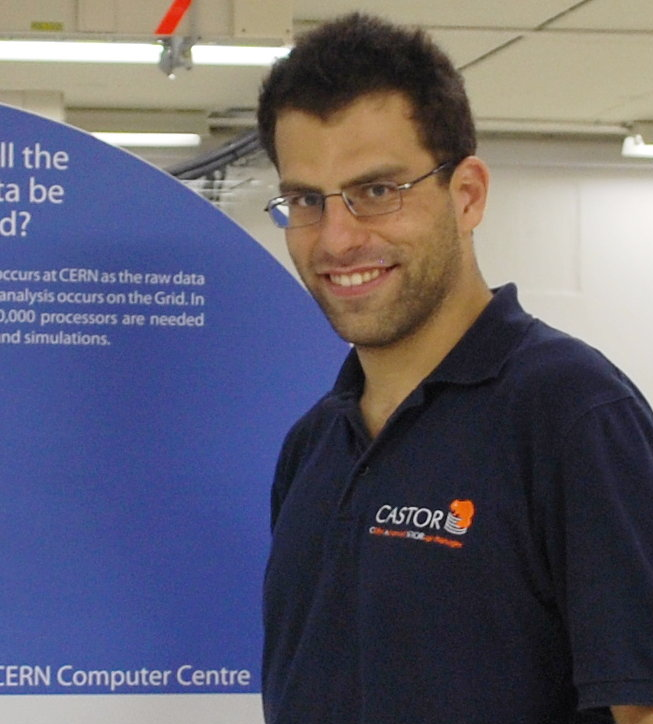
\includegraphics[width=3cm,natwidth=653,natheight=724]{profile.jpg}}
\\
\end{tabularx}


\section{Profile Outline}

Senior software engineer and project manager for a wide variety of applications.
Effective team player in highly-dynamic working environments, very good in
communicating at appropriate technical levels and in writing high quality
reports and presentations, proactive in tackling new tasks.
Enthusiast about emerging technologies such as IoT and BlockChain.
Currently involved in designing, developing and operating Petabyte-scale
data management systems for the High Energy Physics community.


\section{Professional Experience Summary}

\textbf{2008 - present: CERN Staff member, IT Department}\\
Senior developer, project leader, Service Manager for the CASTOR and CERNBox projects\\[.3\baselineskip]
\textbf{2010 - 2015: CERN Staff member, IT Department}\\
Technical Manager of the CERN School of Computing\\[.3\baselineskip]
\textbf{Mar 2005 - Feb 2008: CERN Fellow, IT Department, and Research associate,\\ INFN-CNAF, Bologna, Italy}\\
Developer in the CASTOR project, contact person for the Tier-1 institutes\\[.3\baselineskip]
\textbf{Feb 2004 - Feb 2005: PhD Student, PH Department, CMS experiment}\\
Research and development for the online Data Acquisition system\\[.3\baselineskip]
\textbf{Jul 2001 - Jan 2004: PhD Student, ICAR-CNR, Palermo, Italy}\\
Research and development on Active Networks management\\[.3\baselineskip]
\textbf{1997 - 2008: Freelance IT Consultant}\\
Software engineer and project manager for several web-oriented projects


\section{Detailed Recent Professional Experience}

\subsection{2015 - present}{CASTOR Service Manager, CERN/IT}

Appointed the role of CASTOR Service Manager, responsible for the operations team (about six individuals, two FTEs) to ensure continuous 24/7 support to the experiments' communities and the users for their data taking activities.
CASTOR is a Petabyte-scale Hierarchical Storage Manager (HSM) system designed to archive on tape the physics data at CERN.

\begin{CompactItemize}
\item Ensured smooth data taking operations for all experiments, in particular during the LHC \emph{Run 2}: for instance, the ALICE experiment sustained over 7 GB/s in November 2015, and over 12 PB of data were globally recorded to tape in October 2017
\item Convened annual workshops, monthly phone conferences, and weekly coordination meetings
\item Maintained very good relationships with online and offline computing representatives, contact person for the storage operations team at RAL (UK)
\item Supervised other team members for the daily operations required to run the service
\item Coordinated hardware replacement campaigns with the IT Procurement team while ensuring minimal service disruptions
\item Participated to several selection boards for staff positions in the group
\item Coordinated the software development process and fed back operational requirements
\end{CompactItemize}

\subsection{Dec 2016 - present}{CERNBox, CERN/IT}

Software and service developer for CERNBox, the cloud storage being proposed to all CERN users.

\begin{CompactItemize}
\item Contributed the integration of Microsoft Office Online in CERNBox by designing, implementing and deploying the required connector service
\item Participated in the test of new desktop clients, dealing with the ownCloud core software team
\item Invited to the ownCloud Conference 2017 in N{\"u}rnberg, Germany
\item Contact person for the integration of further Office online platforms, including OnlyOffice and Collabora
\end{CompactItemize}

\subsection{2010 - 2015}{CERN School of Computing Technical Manager, CERN/IT}

Appointed the role of CSC Technical Manager and successfully run 6 main CSCs and 3 \emph{thematic} ones
(\href{http://cern.ch/csc}{http://cern.ch/csc}). The CERN School of Computing aims at promoting
advanced learning and knowledge exchange in scientific computing.

\begin{CompactItemize}
\item Simplified and streamlined the technical infrastructure of the School: introduced
      the use of Virtual Machines for the students' activities and moved heavy-duty exercises to
      high-performance batch nodes hosted at CERN
\item Supported all School-related activities, including mentoring students for the \emph{inverted CSC}s
      and assisting lecturers for the hands-on exercise sessions
\item Supervised a number of Summer Students to support the School's technical infrastructure
\end{CompactItemize}

\subsection{2008 - 2011}{CASTOR SRM Project Leader, CERN/IT}

Project leader of the Storage Resource Manager (SRM) interface for CASTOR, the CERN Advanced STORage
manager system, in the Data and Storage Services group.
SRM is the component responsible for distributing all physics data to the different sites
in the World-wide LHC Computing Grid.

\begin{CompactItemize}
\item Coordinated the contributions of developers at CERN and at RAL (4 individuals, 2 FTEs)
\item Implemented a software development methodology and defined guidelines in order to ensure
  appropriate code reuse across the different CASTOR components
\item Managed the entire software release cycle of the SRM project, including building, packaging and distributing
  new CASTOR SRM releases, as well as defining and implementing the testing and certification procedures
  of the project
\item Participated to several selection boards for staff positions in the group
\end{CompactItemize}

\subsection{2005 - 2015}{Software Engineer, CERN/IT}

Senior developer for the CASTOR project in the Storage group (formerly the Fabric Infrastructure and Operations, Data Management, and Data and Storage Services groups).
The project underwent a major redesign in 2004-2012, and its maturity is now key for effective and low cost operations.

\begin{CompactItemize}
\item Coordinated developments in relation to the different stakeholders, including
  operations teams, experiment representatives, grid middleware developers, and partner Tier-1
  institutes running CASTOR (CNAF in Italy, RAL in UK, and ASGC in Taiwan)
\item Represented the CASTOR project in several workshops and conferences, including the
\emph{IEEE Mass Storage Systems and Technologies} conference, \emph{CHEP}, \emph{HEPiX} workshops, as well as specific events at \emph{ITER} (Cadarache, France) and at Universities
\item Supervised less experienced members of the team, including staff members and technical students
\item Implemented and maintained the framework for database-connected daemons that is used
  across the entire project
\item Maintained a PL/SQL code base designed for high performance and concurrency and developed a
  project-wide process to identify and prevent database deadlocks, which became standard practice in the development team
\item Participated in the definition and in the implementation of the build and release process
  for new CASTOR software versions
\end{CompactItemize}

Software analyst supporting the production operations of CASTOR and the
deployment of the software at the Tier-1 data centres.

\begin{CompactItemize}
\item Expert for the analysis of operational issues in the CASTOR storage service, advising
  the operations team in their deployment and daily operations
\item Participated in the second- and third-level support lines at CERN and for the partner Tier-1
  institutes and taken part in the $24\times7$ \emph{piquet} rota run by the group in 2010-2011
\item Contributed to the setup of the CASTOR system in two Tier-1 centres and trained local
  staff to enable them to run the system independently of the CERN operations team
\item Contributed to bi-weekly phone conferences and face-to-face meetings with all CASTOR stakeholders
\end{CompactItemize}

%\subsection{2002 - 2003}{Freelance IT Consultant}
%
%Software engineer and designer of a web-based system to query the EuroMed PlantBase project
%database (\href{http://www.emplantbase.org}{www.emplantbase.org}), in order to produce
%and publish a taxonomic reference book


\section{Education}

\subsection{2004 - 2005}{PhD Student, CERN/PH}

Joined the PH/CMD group at CERN under the supervision of Dr. L. Orsini. Main research activities:

\begin{CompactItemize}
\item Investigation of Peer-to-Peer architectures for distributed Data Acquisition systems in the
  CMS experiment and implementation of a prototype using the \emph{JXTA}
  technology, an XML-based protocol specification and a framework to build distributed
  Peer-to-Peer applications
\item Participation in the CERN School of Computing 2004 at Vico Equense, Italy
\end{CompactItemize}

\subsection{2001 - 2004}{PhD Student, ICAR-CNR, Italy}

PhD studies at the University of Palermo and at ICAR-CNR (High Performance Computing and Networking Institute,
National Research Council, \href{http://www.icar.cnr.it}{www.icar.cnr.it}), Palermo, under the supervision
of professor S. Gaglio. Main research activities:

\begin{CompactItemize}
\item Multi-tier applications and Prolog-based Artificial Intelligence techniques for Active Networks management.
  Active Networks are a distributed computing paradigm whereby routers deliver traffic based on code directly
  injected into packets, so that an application may dynamically redefine the routing rules
\item Investigations and simulations of multicast protocols for the Steiner Problem in Networks
  to evaluate competitiveness of novel meta-heuristics (Simulated Annealing, Genetic Algorithms)
\item Lecturer on \emph{Network Programming with Java} for the \emph{Computer Networks} course at the University of Palermo
\item Lecturer on \emph{Web systems and Networking} for a number of master-level courses targeted to IT practitioners
\item Participation in the National School of Computer Engineering 2003 at Siena, Italy
\end{CompactItemize}

\subsection{1994 - 2000}{Computer Engineering MSc, University of Palermo, Italy}

Contributed to a number of research projects at the University of Palermo during the undergraduate studies, including:

\begin{CompactItemize}
\item Numeric simulation of the Stochastic Resonance phenomenon in a non-linear bi-stable system,
  in collaboration with the Energy and Physics Applications Department, and presentation of the activity at an international workshop
\item Thesis project at ICAR-CNR, Palermo, about \emph{A Tunable Heuristic for the Multicast
  Tree in Computer Networks}
\end{CompactItemize}

%\subsection{1989 - 1994}{High School Diploma, Don Bosco Ranchibile, Palermo, Italy}
%
%Participated to the national olimpic games on Chemistry, scoring 4th on the non-chemistry high school category


\section{Technical Competencies}

\begin{description}
\item[Languages and technologies]: C++, Python, Java (db interaction, multithreading, web apps),
  shell scripting, SQL (Oracle, SQLServer, MySQL, PostgreSQL), Hadoop, UML, LDAP, Lisp.
\item[Operating systems]: Linux (SL/CentOS and Debian), MS Windows, MacOS X.
\item[Tools]: gdb, valgrind, insure, git, puppet, \LaTeX, Office suites, MS Project.
\end{description}


\section{Languages}

Italian: mother tongue

English, French: professional proficiency


\section{Other Interests and Activities}

Official CERN Guide since 2004 and senior guide (\textquoteleft\emph{conferencier}\textquoteright) since 2011,
for both public and VIP visits in Italian, English, and French.

Skiing instructor as of 2012 with a \emph{Moniteur Federal} license from the French Ski Federation,
contributing to the CERN Ski Club Boureau with the role of secretary in the period 2013 - 2016 and president as of September 2016.

Contact person representing CERN with ASCERI (Association of the Sport Communities of the European Research Institutes, \href{www.asceri.eu}{www.asceri.eu}) since 2014.

Piano, photography, astronomy, hiking, bricolage/IoT.


\section{References}

\begin{tabular*}{\textwidth}{@{\extracolsep{\fill}}p{4cm}p{11cm}}
Alberto Pace \newline \small alberto.pace@cern.ch & Group Leader, IT/Storage group\\
Latchezar Betev \newline \small latchezar.betev@cern.ch & ALICE Offline Computing Coordinator\\
Philippe Charpentier \newline \small philippe.charpentier@cern.ch & LHCb Data Handling Coordinator\\
Fran\c{c}ois Fl\"uckiger \newline \small francois.fluckiger@cern.ch & Former Director, CERN School of Computing\\
%Daniele Bonacorsi \newline \small daniele.bonacorsi@bo.infn.it & Deputy Computing Coordinator, CMS Experiment\\
%Tony Cass \newline \small tony.cass@cern.ch & Group Leader, IT/Database Services\\
%Sergio Cittolin \newline \small sergio.cittolin@cern.ch & Former Project Manager, CMS Trigger and Data Acquisition\\
Nunzio D\textquoteright Addea \newline \small n.daddea@itia.mi.cnr.it & Former Research Director,
Istituto di Tecnologie Industriali e \newline Automazione, CNR, Milano, Italy\\
\end{tabular*}

% The section headings
\renewcommand{\section}[2]%
    {\vspace{1.3\baselineskip}%
     \hspace{0in}%
     {\raggedright \scshape #2}\\[-0.15\baselineskip]%
        \rule{\columnwidth}{1pt}%
     \vspace{-.7\baselineskip}%
     \hspace{0in}
    }

\pagebreak

\renewcommand{\refname}{Selected Publications}
% grep '@' cv.bib | cut -d\{ -f 2 | cut -d, -f 1 | awk '{print "\\nocite{" $1 "}"}' 
\begin{bibunit}[cv]
\nocite{CHEP17}
\nocite{CHEP15}
\nocite{EspinalCHEP13}
\nocite{CHEP13}
\nocite{CHEP12}
\nocite{JSAC08}
\nocite{CastorMSST07}
\nocite{SRMMSST07}
\nocite{CHEP07}
%\nocite{Netcoop07}
\nocite{Infocom07}
\nocite{PhDThesis}
\nocite{ICCS04}
\nocite{IASTED03}
%\nocite{IWAN02}
\nocite{GIREP98}
\putbib[cv]
\end{bibunit}

\pagebreak

\renewcommand{\refname}{Selected Presentations}
\begin{bibunit}[cv]
\nocite{CS3W18}
\nocite{HEPiX17}
\nocite{ownCloud17}
\nocite{Unife16}
\nocite{CASTORF2FCh}
\nocite{ITER12}
\nocite{HEPiX11}
\nocite{UnifeUnipa09}
\nocite{GDB09}
\nocite{HEPiX08}
\nocite{DBW08}
\nocite{Parallel08}
\nocite{LHCCReview07}
%\nocite{DReview06}
%\nocite{Review06}
\nocite{CASTORF2F}
\nocite{CMS04}
\putbib[cv]
\end{bibunit}

\end{document}
